% Copyright 2004 by Till Tantau <tantau@users.sourceforge.net>.
%
% In principle, this file can be redistributed and/or modified under
% the terms of the GNU Public License, version 2.
%
% However, this file is supposed to be a template to be modified
% for your own needs. For this reason, if you use this file as a
% template and not specifically distribute it as part of a another
% package/program, I grant the extra permission to freely copy and
% modify this file as you see fit and even to delete this copyright
% notice. 

% \UseRawInputEncoding
\documentclass{beamer}

% There are many different themes available for Beamer. A comprehensive
% list with examples is given here:
% http://deic.uab.es/~iblanes/beamer_gallery/index_by_theme.html
% You can uncomment the themes below if you would like to use a different
% one:
%\usetheme{AnnArbor}
%\usetheme{Antibes}
%\usetheme{Bergen}
%\usetheme{Berkeley}
%\usetheme{Berlin}
%\usetheme{Boadilla}
%\usetheme{boxes}
%\usetheme{CambridgeUS}
%\usetheme{Copenhagen}
%\usetheme{Darmstadt}
%\usetheme{default}
%\usetheme{Frankfurt}
%\usetheme{Goettingen}
%\usetheme{Hannover}
%\usetheme{Ilmenau}
%\usetheme{JuanLesPins}
%\usetheme{Luebeck}
\usetheme{Madrid}
%\usetheme{Malmoe}
%\usetheme{Marburg}
%\usetheme{Montpellier}
%\usetheme{PaloAlto}
%\usetheme{Pittsburgh}
%\usetheme{Rochester}
%\usetheme{Singapore}
%\usetheme{Szeged}
%\usetheme{Warsaw}

\usepackage{pgfgantt}
\usepackage{todonotes}
\usepackage{media9}
\usepackage{fontawesome5}
\usepackage{subfigure}
\usepackage{booktabs,array}
\usepackage{tabulary}
\usepackage{caption}
\usepackage{graphicx}
\usepackage{siunitx}
\usepackage{arydshln}

\usepackage[ruled, vlined, linesnumbered]{algorithm2e} % For algorithms

\usepackage{amsmath} % For typesetting math

% Customize Warsaw color 
\setbeamercolor*{palette primary}{use=structure,fg=white,bg=red!50!black}
\setbeamercolor*{palette secondary}{use=structure,fg=white,bg=red!60!black}
\setbeamercolor*{palette tertiary}{use=structure,fg=white,bg=red!70!black}

% Customize Warsaw block title and background colors
\setbeamercolor{block title}{bg=red!50!black,fg=white}

\setbeamertemplate{bibliography item}{\insertbiblabel}  % insert bibliography numbers instead of symbol
\setbeamertemplate{caption}[numbered] % adds the figure or table number to the caption.


\title[HIL Plant Modeling]{Hardware-in-the-Loop Plant Modeling for Autonomous
  Vehicle}

% % A subtitle is optional and this may be deleted
\subtitle{Modeling, Simulation, and Testing}

\author[H.~Grady, N.~Nauman]{Hannah~Grady \and Nicholas~Nauman 
\linebreak Advisor:~Dr.~Suruz~Miah}
% - Give the names in the same order as the appear in the paper.
% - Use the \inst{?} command only if the authors have different
%   affiliation.

\institute[Bradley University] % (optional, but mostly needed)
{
  Department of Electrical and Computer Engineering\\
  Bradley University\\
  1501 W. Bradley Avenue\\
  Peoria, IL, 61625, USA
}
% - Use the \inst command only if there are several affiliations.
% - Keep it simple, no one is interested in your street address.

\date[October~7,~2021]{Thursday, October~7,~2021}

% - Either use conference name or its abbreviation.
% - Not really informative to the audience, more for people (including
%   yourself) who are reading the slides online

\logo{\hfill\href{http://www.bradley.edu}{
\includegraphics[width=0.75cm]{figs/logoBU1-Print}}}  % place logo in every page 


% \subject{Mobile Robot Localization}
% This is only inserted into the PDF information catalog. Can be left
% out. 

% If you have a file called "university-logo-filename.xxx", where xxx
% is a graphic format that can be processed by latex or pdflatex,
% resp., then you can add a logo as follows:

% \pgfdeclareimage[height=0.5cm]{university-logo}{university-logo-filename}
% \logo{\pgfuseimage{university-logo}}

% Delete this, if you do not want the table of contents to pop up at
% the beginning of each subsection:
\AtBeginSubsection[]
{
  \begin{frame}<beamer>{Outline}
    \tableofcontents[currentsection,currentsubsection]
  \end{frame}
}

% Delete this, if you do not want the table of contents to pop up at
% the beginning of each section:
\AtBeginSection[]
{
  \begin{frame}<beamer>{Outline}
    \tableofcontents[currentsection]
  \end{frame}
}

% Let's get started
\begin{document}

\begin{frame}
  \titlepage
\end{frame}

\begin{frame}{Outline} 
  \tableofcontents%[pausesections]
  % You might wish to add the option [pausesections]
\end{frame}

% Section and subsections will appear in the presentation overview
% and table of contents.
\section{Introduction}

\begin{frame}{Introduction}{}
    \begin{block}{Applications of Autonomous Vehicles}
    	\begin{itemize}
    		\item Autonomous vehicles are being developed by many companies for commercial and personal use
    		\item Modeling the steering system for autonomous vehicles is a challenging task
     		\item Models for autonomous vehicle subsystems must be very accurate due to safety factors
		\end{itemize}
    \end{block}
        \begin{figure}
			\centering
			\begin{minipage}[t]{0.4\textwidth}
				\centering
				\includegraphics[height=1.5cm]{figs/img/autonomousVehiclesAStuff}
				\caption{AutonomouStuff Vehicle Fleet\textsuperscript{a}}
				\label{fig:fleet}
			\end{minipage}
			\begin{minipage}[t]{0.4\textwidth}
				\centering
				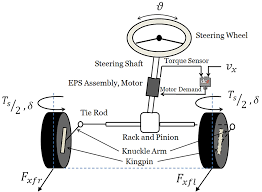
\includegraphics[height=1.5cm]{figs/img/autonomousVehiclesSteering}
				\caption{Autonomous Vehicle Steering System\textsuperscript{b}}
				\label{fig:steerSystem}
			\end{minipage}
        \end{figure}
    \begin{tiny}
		\textsuperscript{a}https://hexagonpositioning.com/pi-brands/autonomoustuff\\\textsuperscript{b}https://www.autonews.com/article/20181105/OEM10/181109921/delphi-s-pace-award-winning-e-steer-an-autonomous-vehicle-building-block
    \end{tiny}
\end{frame}

\begin{frame}{Problem Statement}
  \begin{block}{Problem Statement}
    \begin{large}
      Model vehicle subsystems for a Lexus platform.
 \begin{itemize}
          \item Steering Model
          \item Acceleration Model
          \item Brake Model
          \item Shift Model
          \item Speed Model
          \item Speed Control Model
        \end{itemize} 
    \end{large}
  \end{block}
  \pause
  \begin{block}{Proposed Solution}
    \begin{large}
      A potential solution is to develop conventional System Identification techniques for modeling subsystems using available raw data.  
    \end{large}
  \end{block}
\end{frame}

%----------------------------------

\section{Literature Review}

\begin{frame}{Literature Review}
  \begin{block}{Existing Solutions}
 \begin{itemize}
        \item Use of System Identification Toolbox in Matlab to create models from data~\cite{Adnan2010}
	 \begin{itemize}
		    \tiny
		    		\item Offers a variety of model choices
				\item Needs a large amount of raw data to produce an accurate model
	\end{itemize}
	\item Third order ARMAX model creates models using traditional methods of analysis~\cite{Li1999}
	 \begin{itemize}
		    \tiny
		    		\item Allows the use of traditional analysis methods to create a model 
				\item More room for error during calculations
	\end{itemize}
	\item Steer-By-Wire method as a system model~\cite{Saruchi2015}
	 \begin{itemize}
		    \tiny
		    		\item Can model systems with small non-linearities 
				\item Mechanical components replaced by electrical components 
	\end{itemize}
	\item Authors in~\cite{Hussain2011} illustrate identification of multiple-input single-output model for maximum power point tracking of photovoltaic system.  
	\begin{itemize}
	\tiny
		\item Fourth order ARX model ended up giving the best fit
	\end{itemize}
\end{itemize}
  \end{block}
    % \begin{figure}[b]
    %     \centering
    %     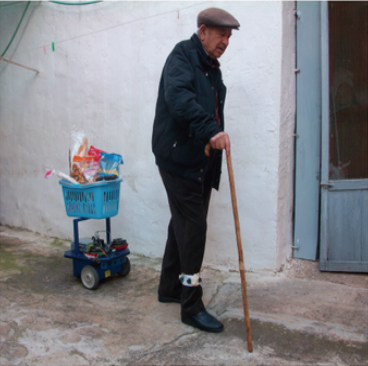
\includegraphics[width=0.45\textwidth]{figs/img/CompaRob}
    %     \caption{CompaRob}
    %     %\label{fig:sysBlockDiag}
    % \end{figure}
\end{frame}


%----------------------------------

\section{System Requirements}

\begin{frame}{System Requirements}
  \begin{block}{Specifications}
    The vehicle plant model will fulfill the requirements listed below:
\begin{itemize}
    \item The resulting plant model will consist of accurate subsystem models
    \item The subsystems can be used to create a HIL testbench
    \item The steering model can handle very small changes in steering angles
    \begin{itemize}
    		\item smooth out any non-linear discontinuities that would normally be measured by the steering motor, especially for small changes in the steering angle, depicted in \autoref{fig:nonlinGraph}.
    \end{itemize}
\end{itemize}
\begin{figure}[h]
    \centering
    \captionsetup{justification=centering, margin=3cm}
    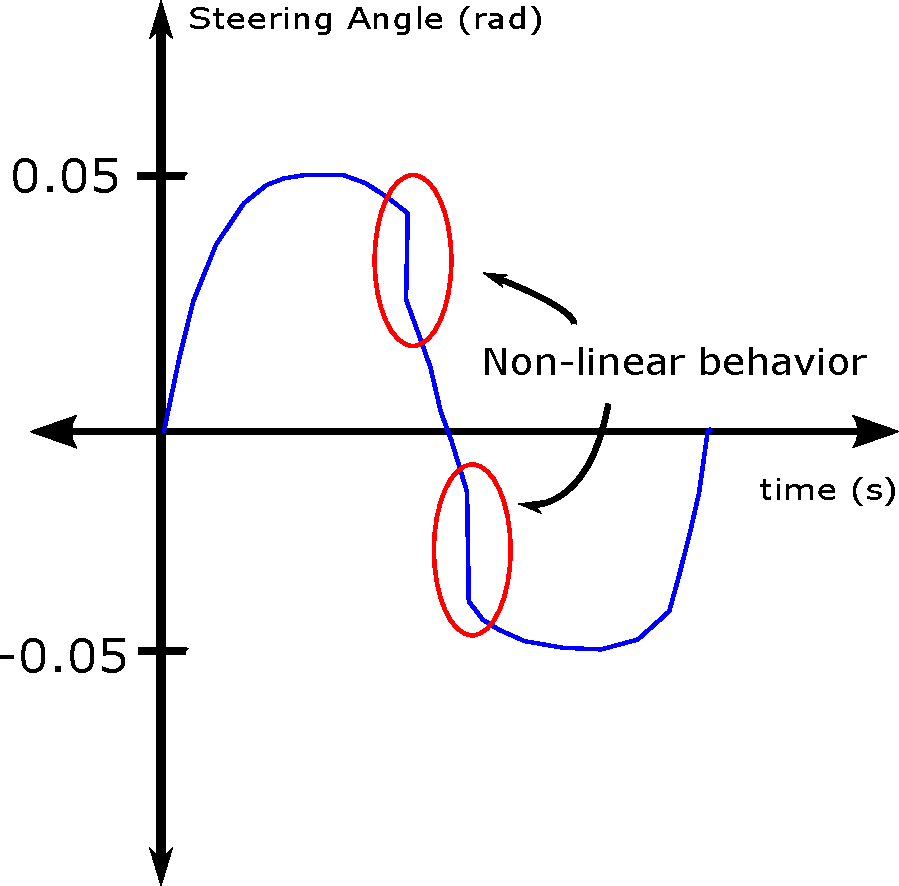
\includegraphics[width=1in]{figs/inkscape/nonlinearBehavior}
    \caption{Steering Non-linear Behavior}
    \label{fig:nonlinGraph}
\end{figure}
  \end{block}
\end{frame}

%--------------------------------

\section{System Architecture}

\begin{frame}{System Architecture}
  \begin{block}{System Architecture}
 \begin{itemize}
        \item The overall system architecture of this project consists of six subsystems which are the steering, acceleration, brake, speed, shift, and cruise control systems
\end{itemize}
  \end{block}
\end{frame}

\begin{frame}
\begin{minipage}[t]{0.48\linewidth}
\tiny
	\begin{block}{System Inputs}
		\begin{itemize}
			\tiny
		    \item Steering Model
		    \begin{itemize}
		    \tiny
		    		\item Torque Voltages
		    		\begin{itemize}
		    		\tiny
		    			\item Desired Steering Wheel Angle
		    			\item Actual Steering Wheel Angle
		    		\end{itemize}
		    \end{itemize}
		    \item Acceleration Model
		    \begin{itemize}
		    \tiny
		    		\item Acceleration Pedal Voltages
		    \end{itemize}
		    \item Brake Model
		    \begin{itemize}
		    \tiny
		    		\item Brake Pedal Pressure Voltages
		    		\item Brake Pedal Stroke Voltages 
		    		\item Brake Pedal On/Off Switch
		    \end{itemize}
		    \item Shift Model
		    \begin{itemize}
		    \tiny
		    		\item Desired Shift Gear
		    \end{itemize}
		    \item Speed Model
		    \begin{itemize}
		    \tiny
		    		\item Acceleration Pedal Position
		    		\item Brake Pedal Position
		    		\item Shifter Actual Gear
		    \end{itemize}
		    \item Speed Control Model
		    \begin{itemize}
		    \tiny
		    		\item Desired Vehicle Speed
		    \end{itemize}
		\end{itemize}
	\end{block}
\end{minipage}%
\hfill%
\begin{minipage}[t]{0.48\linewidth}
\begin{block}{System Outputs}
		\begin{itemize}
			\tiny
		    \item Steering Model
		    \begin{itemize}
		    \tiny
		    		\item Wheel Angle
		    		\item Actual Steering Angle
		    \end{itemize}
		    \item Acceleration Model
		    \begin{itemize}
		    \tiny
		    		\item Acceleration Pedal Position
		    \end{itemize}
		    \item Brake Model
		    \begin{itemize}
		    \tiny
		    		\item Brake Pedal Position
		    		\item Brake Pressed
		    \end{itemize}
		    \item Shift Model
		    \begin{itemize}
		    \tiny
		    		\item Actual Shift Gear
		    \end{itemize}
		    \item Speed Model
		    \begin{itemize}
		    \tiny
		    		\item Vehicle Speed
		    \end{itemize}
		    \item Speed Control Model
		    \begin{itemize}
		    \tiny
		    		\item Vehicle Speed
		    \end{itemize}
		\end{itemize}
	\end{block}
\end{minipage}
\end{frame}


\begin{frame}
\centering
\includegraphics[width=.45\linewidth]{figs/inkscape/steeringModelArchitecture}\quad%
\begin{minipage}[b][0.4\textheight][c]{.45\linewidth} \begin{enumerate} \item Steering System \item Brake System \item Acceleration System \end{enumerate} \end{minipage}\\[1em]
\includegraphics[width=.45\linewidth]{figs/inkscape/brakeModelArchitecture}\quad%
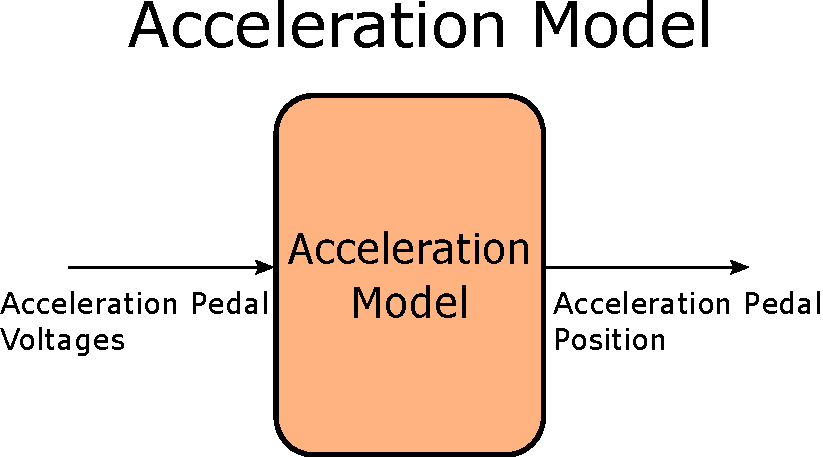
\includegraphics[width=.45\linewidth]{figs/inkscape/accelerationModelArchitecture}
\end{frame}


\begin{frame}
\centering
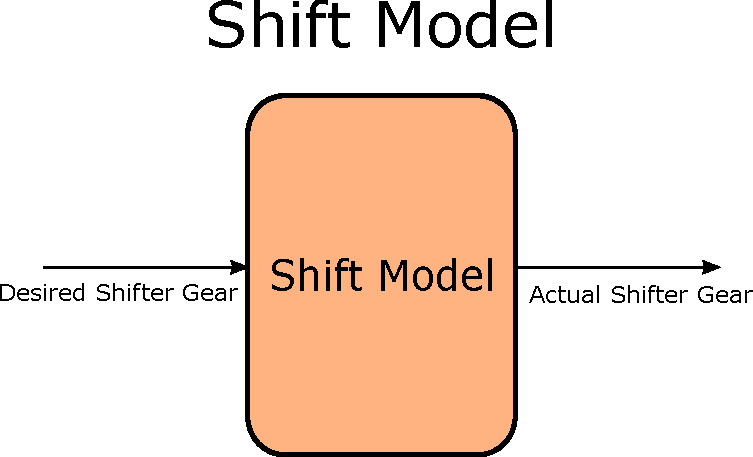
\includegraphics[width=.45\linewidth]{figs/inkscape/shiftModelArchitecture}\quad%
\begin{minipage}[b][0.4\textheight][c]{.45\linewidth} \begin{enumerate} \item Shift System \item Speed Control System \item Speed System \end{enumerate} \end{minipage}\\[1em]
\includegraphics[width=.45\linewidth]{figs/inkscape/speedControlModelArchitecture}\quad%
\includegraphics[width=.45\linewidth]{figs/inkscape/speedModelArchitecture}
\end{frame}


\begin{frame}
\begin{figure}[h]
    \centering
    \captionsetup{justification=centering, margin=3cm}
    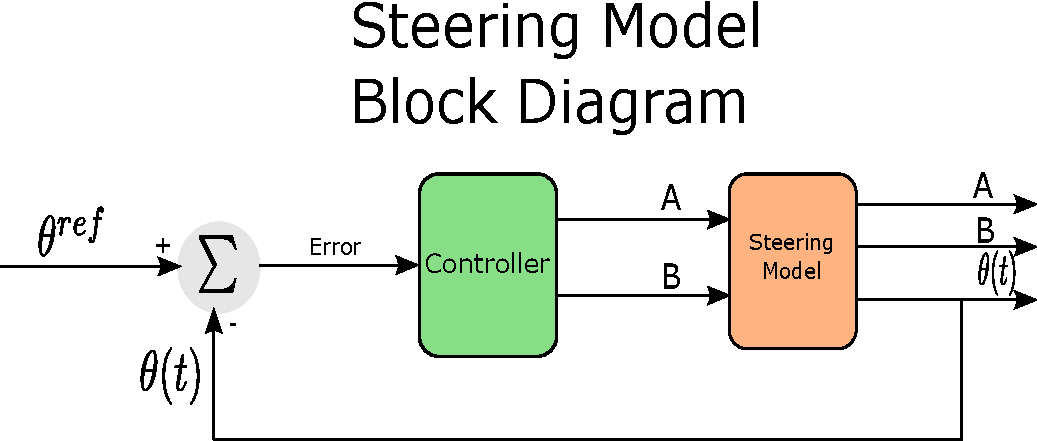
\includegraphics[width=4in]{figs/inkscape/steeringModelBlockDiagram}
    \caption{Steering System Block Diagram}
    \label{fig:steerBlockDiag}
\end{figure}
\end{frame}

%----------------------------------

\section{System Identification}

\begin{frame}{System Identification}
  \begin{block}{System Identification}
 \begin{itemize}
        \item System identification is the process of developing mathematical models for a dynamic system using the measurement of input and output signals of that system. The goal of the system identification methodology is to get an accurate estimation of the system response to any given input. Mathworks' MATLAB has the system identification toolbox, where a few existing examples demonstrate the working principle of this toolbox.
\end{itemize}
  \end{block}
\end{frame}

\subsection{Preliminary Work}

\begin{frame}{Preliminary Work}
  \begin{block}{Preliminary Work}
 \begin{itemize}
        \item Documentation on MATLAB's System Identification Toolbox and tutorials
        \item Literature Review 
        \item Data Collection for steering, braking and acceleration subsystems
\end{itemize}
  \end{block}
  \begin {block}{Modeling}
  \begin{itemize}
  	\item All modeling of vehicle subsystems will be done using MATLAB's System Identification Toolbox feature. The subsystems can be grouped into four different categories: Single-Input-Single-Output, Multiple-Input-Multiple-Output, Single-Input-Multiple-Output, and Multiple-Input-Single-Output. 
  	\end{itemize}
  	\end{block}
\end{frame}

%----------------------------------
\subsection{Design}

\begin{frame}{Design}
	\begin{block}{}
		Each subsystem that we are modeling are set up in a similar manner. In manual mode, the torque voltages that control each subsystem are sent by the electronic control unit (ECU). In order to control the vehicle autonomously, the vehicle subsystem switches to by-wire mode. In by-wire mode, the torque voltages from the ECU are discarded by open-circuiting the motors that control each subsystem. Instead, controllers built by AutonomouStuff send the torque voltages to the motor using relays.
	\end{block}
\end{frame}

%----------------------------------
\subsection{Parts List}

\begin{frame}{Parts List}
  \begin{block}{Software and Hardware}
 \begin{itemize}
        \item Software
        \begin{itemize}
        \small
        \item MATLAB's System Identification Toolbox
        \item Vector CANAlyzer
        \end{itemize}
	\item Hardware
	\begin{itemize}
	\small
	\item Laptop
	\item PAC Mod
	\item CAN Case 
	\item CAN Bus
	\end{itemize}
\end{itemize}
  \end{block}
\end{frame}

%----------------------------------
\subsection{Modeling}

\begin{frame}{Model Equations}
	\begin{block}{}
		\begin{itemize}
			\item Transfer Function Model: 
			\begin{equation}
				\frac{Y(s)}{U_A(s)} = \frac{b_{n}*s^{n} + b_{n-1}*s^{n-1} + ... + b_1*s + b_0}{a_{m}*s^{m} + a_{m-1}*s^{m-1} + ... + a_1*s + a_0}
			\end{equation}
			where m = number of poles and n = number of zeros
			\item ARX Model: 
			\begin{equation}
				A(z)*y(t) = B(z)*u(t) + e(t)
			\end{equation}
		\end{itemize}
	\end{block}
\end{frame}

%----------------------------------
\section{Validation and Testing}

\begin{frame}{Simulation Results}
  \begin{block}{Steering System}
 \begin{itemize}
	\item Best fit percentage of the by-wire steering estimated model is 85.54
	\item Best fit percentage of the manual steering estimated model is 90.27
 \end{itemize}
 \begin{figure}
    \centering
    \begin{minipage}{0.45\textwidth}
        \centering
        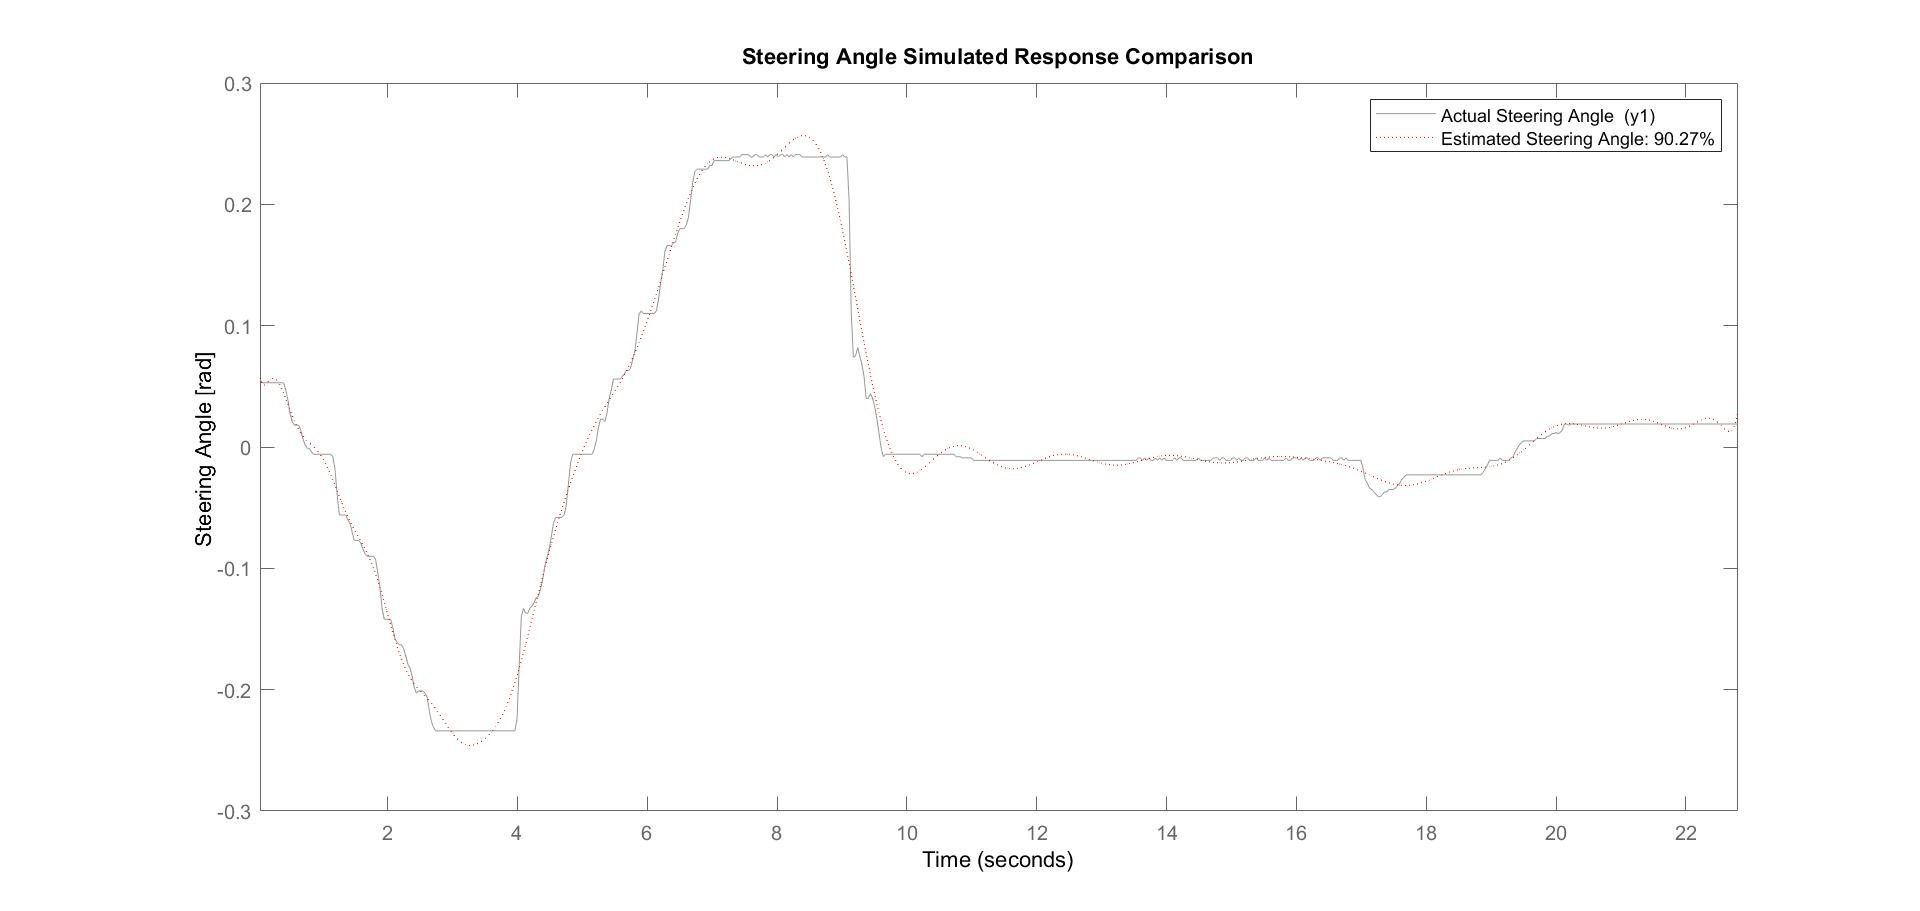
\includegraphics[width=0.9\textwidth]{figs/img/byWireSteeringTransferFunctionModel} % first figure itself
        \caption{Output of Estimated By-Wire System Model}
        \label{fig:byWireSteerModel}
    \end{minipage}\hfill
    \begin{minipage}{0.45\textwidth}
        \centering
        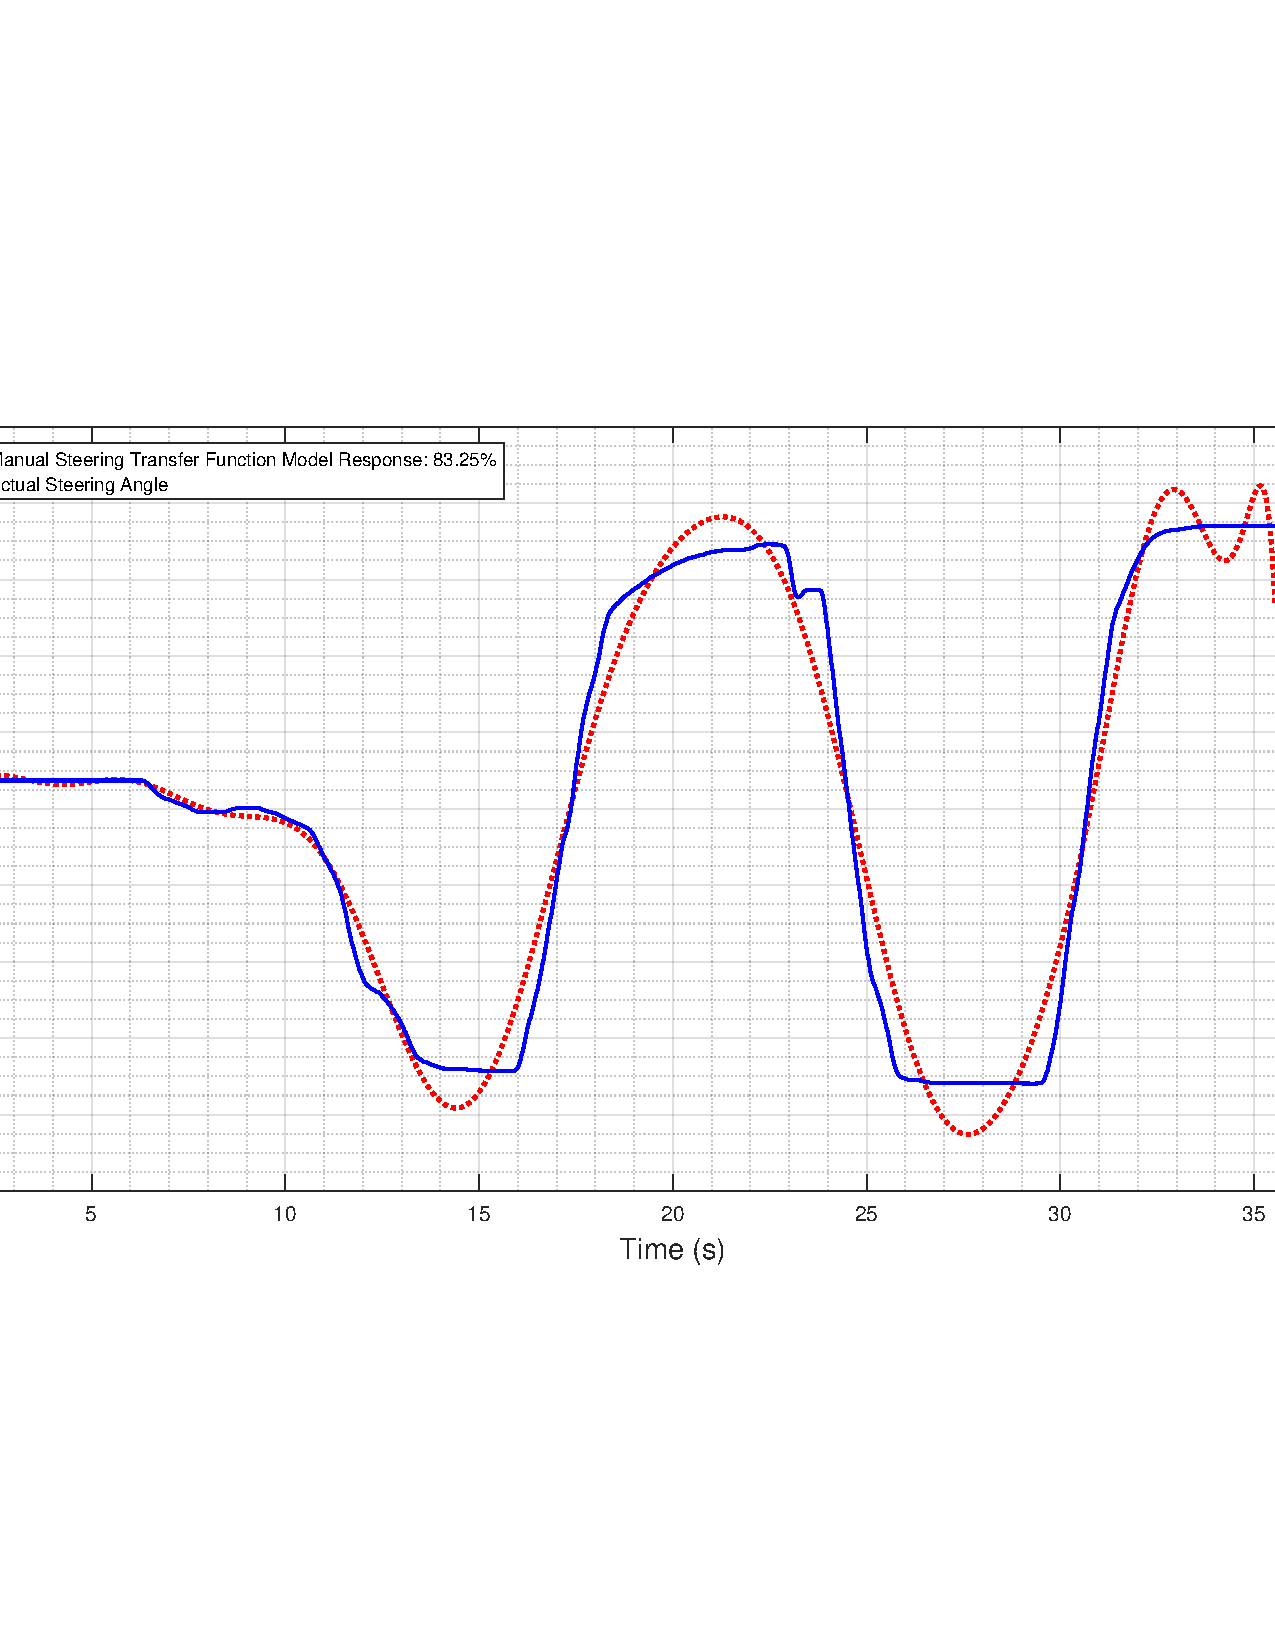
\includegraphics[width=0.9\textwidth]{figs/img/manualSteeringTransferFunctionModel} % second figure itself
        \caption{Output of Estimated Manual System Model}
        \label{fig:manualSteerModel}
    \end{minipage}
\end{figure}
  \end{block}
\end{frame}

\begin{frame}{By-Wire Steering System Transfer Function}
\begin{minipage}[t]{0.48\linewidth}
	\begin{block}{Torque A}
		\tiny
		\begin{tabular}{ cc }   % top level tables, with 2 columns
			% leftmost table of the top level table
			\begin{tabular}{ |c|c| } 
				\hline
				b_0 & 3.44E-16 \\
				b_1 & -2.203E-15 \\
				b_2 & 1.24E-13 \\
				b_3 & 5.975E-13 \\
				b_4 & 3.001E-12 \\
				b_5 & 5.23E-12 \\
				\hline
			\end{tabular} &  % starting rightmost sub table
			% table 2
			\begin{tabular}{ |c|c| } 
				\hline
				a_0 & 1.949E-16 \\
				a_1 & 1.455E-14 \\
				a_2 & 8.797E-13 \\
				a_3 & 2.304E-11 \\
				a_4 & 9.041E-10 \\
				a_5 & 9.01E-9 \\
				a_6 & 2.714E-7 \\
				a_7 & 9.241E-7 \\
				a_8 & 1.946E-5 \\
				a_9 & 3.889E-5 \\
				a_{10} & 0.0005721 \\
				a_{11} & 0.0008035 \\
				a_{12} & 0.008695 \\
				a_{13} & 0.008922 \\
				a_{14} & 0.07499 \\
				a_{15} & 0.05422 \\
				a_{16} & 0.3631 \\
				a_{17} & 0.1693 \\
				a_{18} & 0.9394 \\
				a_{19} & 0.2118 \\
				a_{20} & 1 \\
				\hline
			\end{tabular} \\
		\end{tabular}
	\end{block}
\end{minipage}%
\hfill%
\begin{minipage}[t]{0.48\linewidth}
	\begin{block}{Torque B}
		\tiny
		\begin{tabular}{ cc }   % top level tables, with 2 columns
			% leftmost table of the top level table
			\begin{tabular}{ |c|c| } 
				\hline
				b_0 & -6.645E-15 \\
				b_1 & 2.161E-14 \\
				b_2 & -2.605E-14 \\
				b_3 & -4.744E-13 \\
				b_4 & -1.813E-13 \\
				b_5 & -4.858E-12 \\
				\hline
			\end{tabular} &  % starting rightmost sub table
			% table 2
			\begin{tabular}{ |c|c| } 
				\hline
				a_0 & 2.92E-15 \\
				a_1 & 2.758E-13 \\
				a_2 & 1.761E-11 \\
				a_3 & 4.228E-10 \\
				a_4 & 1.422E-8 \\
				a_5 & 1.561E-7 \\
				a_6 & 1.501E-6 \\
				a_7 & 8.426E-6 \\
				a_8 & 5.981E-5 \\
				a_9 & 0.0002016 \\
				a_{10} & 0.001226 \\
				a_{11} & 0.002649 \\
				a_{12} & 0.01456 \\
				a_{13} & 0.02044 \\
				a_{14} & 0.104 \\
				a_{15} & 0.09228 \\
				a_{16} & 0.4417 \\
				a_{17} & 0.2257 \\
				a_{18} & 1.025 \\
				a_{19} & 0.2305 \\
				a_{20} & 1 \\
				\hline
			\end{tabular} \\
		\end{tabular}
	\end{block}
\end{minipage}
\end{frame}

\begin{frame}{Manual Steering System Transfer Function}
\begin{minipage}[t]{0.48\linewidth}
	\begin{block}{Torque A}
		\tiny
		\begin{tabular}{ cc }   % top level tables, with 2 columns
			% leftmost table of the top level table
			\begin{tabular}{ |c|c| } 
				\hline
				b_0 & 6.516E4 \\
				b_1 & -2.944E5 \\
				b_2 & 2.328E5 \\
				b_3 & -2.487E5 \\
				b_4 & 8.25E4 \\
				b_5 & -3.038E4 \\
				\hline
			\end{tabular} &  % starting rightmost sub table
			% table 2
			\begin{tabular}{ |c|c| } 
				\hline
				a_0 & 1.224E5 \\
				a_1 & 4.227E5 \\
				a_2 & 2.202E6 \\
				a_3 & 3.54E6 \\
				a_4 & 7.98E6 \\
				a_5 & 7.62E5 \\
				a_6 & 1.071E7 \\
				a_7 & 6.745E6 \\
				a_8 & 6.85E6 \\
				a_9 & 3.006E6 \\
				a_{10} & 2.365E6 \\
				a_{11} & 7.37E5 \\
				a_{12} & 4.669E5 \\
				a_{13} & 1.021E5 \\
				a_{14} & 5.319E4 \\
				a_{15} & 7752 \\
				a_{16} & 3353 \\
				a_{17} & 287.5 \\
				a_{18} & 102.4 \\
				a_{19} & 3.653 \\
				a_{20} & 1 \\
				\hline
			\end{tabular} \\
		\end{tabular}
	\end{block}
\end{minipage}%
\hfill%
\begin{minipage}[t]{0.48\linewidth}
	\begin{block}{Torque B}
		\tiny
		\begin{tabular}{ cc }   % top level tables, with 2 columns
			20th Order Transfer Function Model			
			% leftmost table of the top level table
			\begin{tabular}{ |c|c| } 
				\hline
				b_0 & 1.209E4 \\
				b_1 & 1.855E5 \\
				b_2 & -2.801E5 \\
				b_3 & 4.72E5 \\
				b_4 & -3.976E4 \\
				b_5 & 7.693E4 \\
				\hline
			\end{tabular} &  % starting rightmost sub table
			% table 2
			\begin{tabular}{ |c|c| } 
				\hline
				a_0 & 4.687E4 \\
				a_1 & 7.037E5 \\
				a_2 & 2.624E6 \\
				a_3 & 6.133E6 \\
				a_4 & 1.197E7 \\
				a_5 & 1.487E7 \\
				a_6 & 1.887E7 \\
				a_7 & 1.446E7 \\
				a_8 & 1.314E7 \\
				a_9 & 7.01E6 \\
				a_{10} & 4.79E6 \\
				a_{11} & 1.886E6 \\
				a_{12} & 9.836E5 \\
				a_{13} & 2.937E5 \\
				a_{14} & 1.149E5 \\
				a_{15} & 2.617E4 \\
				a_{16} & 7205 \\
				a_{17} & 1232 \\
				a_{18} & 200 \\
				a_{19} & 23.54 \\
				a_{20} & 1 \\
				\hline
			\end{tabular} \\
		\end{tabular}
	\end{block}
\end{minipage}
\end{frame}

\begin{frame}{Simulation Results}
  \begin{block}{Acceleration System}
 \begin{itemize}
	\item Best fit percentage of the by-wire acceleration estimated model is 97.69
	\item Best fit percentage of the manual acceleration estimated model is 98.3
 \end{itemize}
 \begin{figure}
    \centering
    \begin{minipage}{0.45\textwidth}
        \centering
        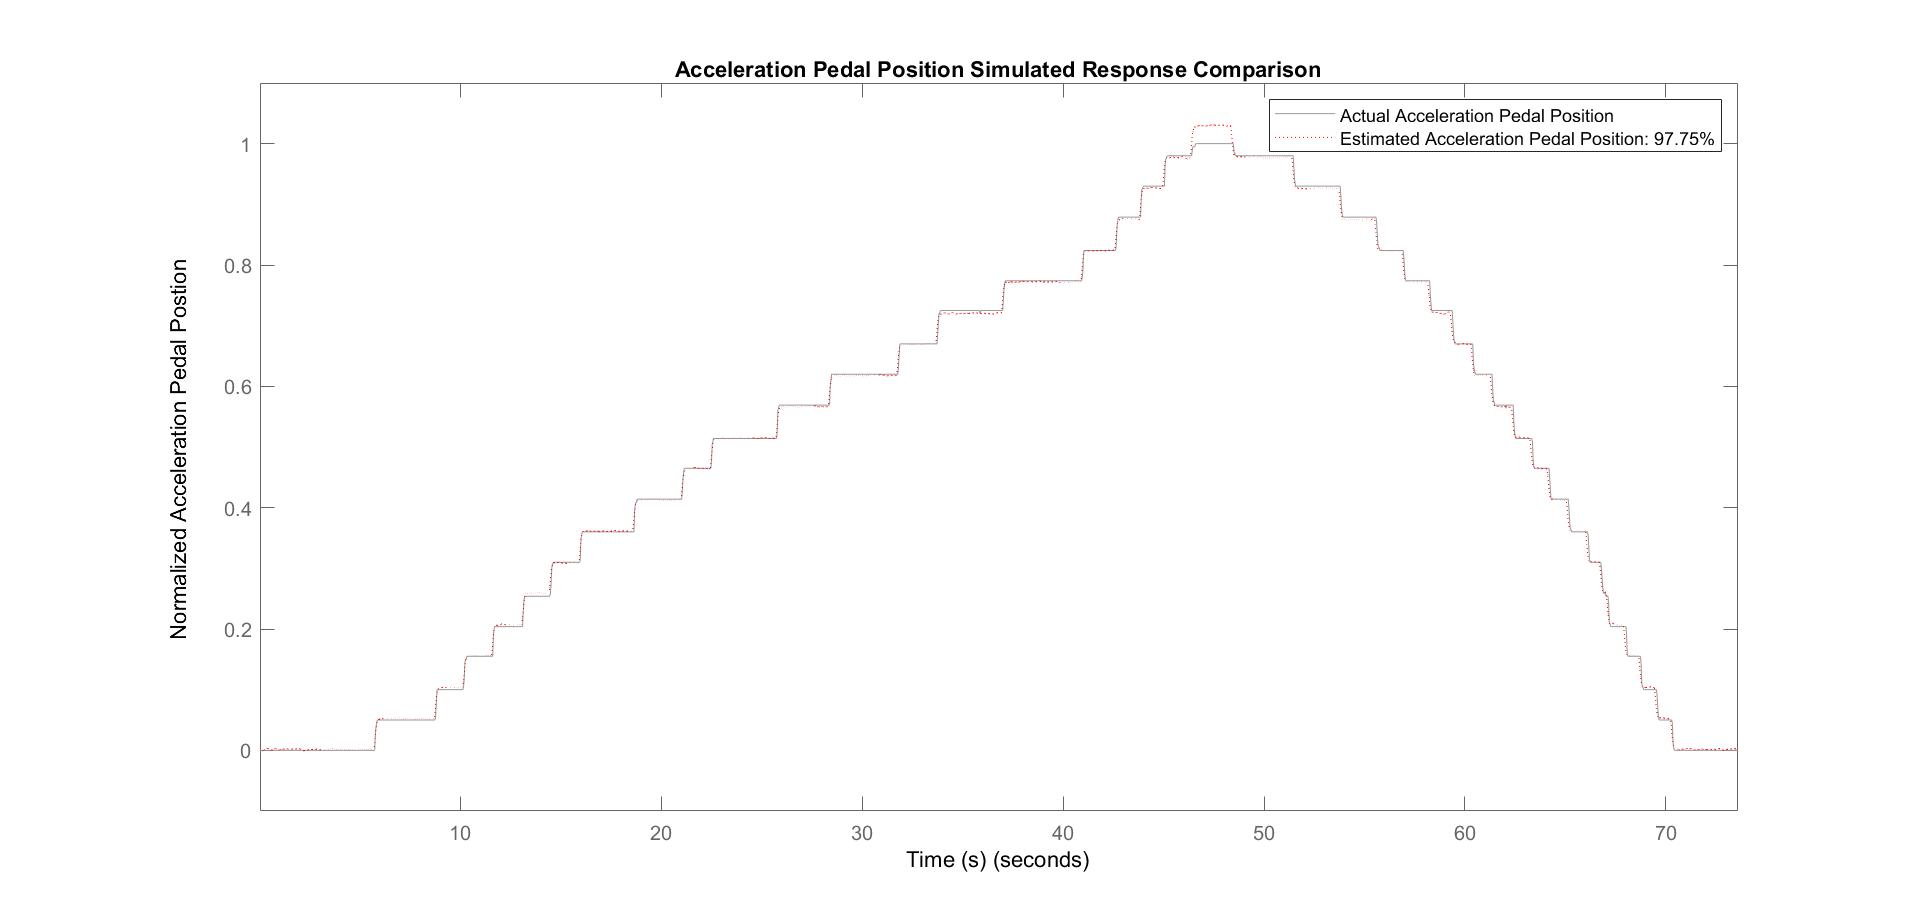
\includegraphics[width=0.9\textwidth]{figs/img/byWireAccelArxModel} % first figure itself
        \caption{Output of Estimated By-Wire System Model}
        \label{fig:byWireAccelModel}
    \end{minipage}\hfill
    \begin{minipage}{0.45\textwidth}
        \centering
        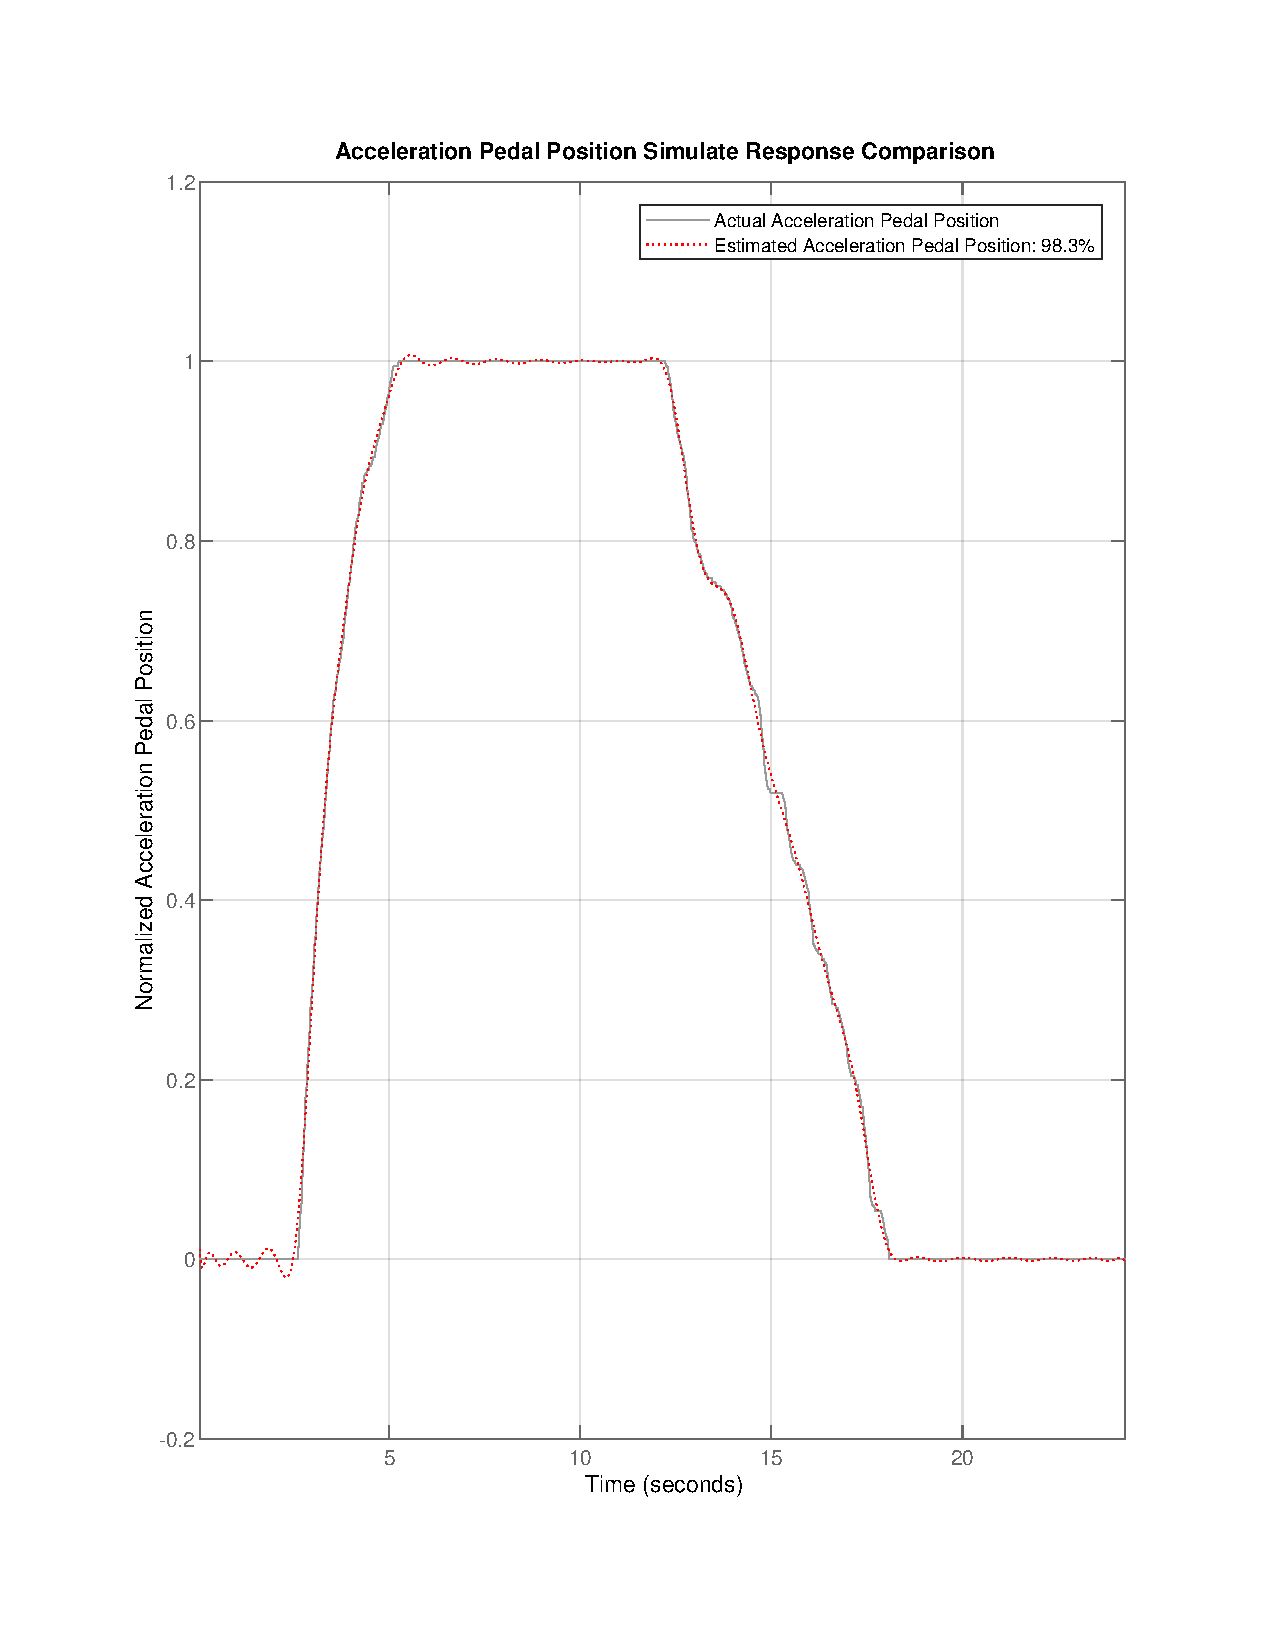
\includegraphics[width=0.9\textwidth]{figs/img/manualAccelTransferFunctionModel} % second figure itself
        \caption{Output of Estimated Manual System Model}
        \label{fig:manualAccelModel}
    \end{minipage}
\end{figure}
  \end{block}
\end{frame}

\begin{frame}{By-Wire Acceleration System Transfer Function}
	\begin{block}{Fourth-Order ARX Model}
		\begin{equation}
			A(z)*y(t) = B(z)*u(t) + e(t)
		\end{equation}
		%
		where, 
		%
		\begin{equation}
			A(z) = 1 - 1.018*z^{-1} - 0.002901*z^{-2} + 0.4631*z^{-3} - 0.2038*z^{-4}
		\end{equation}
		\begin{equation}
			B_1(z) = -0.0207 - 0.01912*z^{-1} - 0.02159*z^{-2} - 0.03307*z^{-3}
		\end{equation}
		\begin{equation}
			B_2(z) = 0.02017 + 0.01833*z^{-1} + 0.09461*z^{-2} + 0.05683*z^{-3}
		\end{equation}
	\end{block}
\end{frame}

\begin{frame}{Manual Acceleration System Transfer Function}
\begin{minipage}[t]{0.48\linewidth}
	\begin{block}{Torque A}
		\tiny
		\begin{tabular}{ cc }   % top level tables, with 2 columns
			% leftmost table of the top level table
			\begin{tabular}{ |c|c| } 
				\hline
				b_0 & -5.741E6 \\
				b_1 & -2.644E7 \\
				b_2 & -2.797E6 \\
				b_3 & -1.304E7 \\
				b_4 & -3.203E6 \\
				b_5 & -1.159E6 \\
				b_6 & -5.519E5 \\
				\hline
			\end{tabular} &  % starting rightmost sub table
			% table 2
			\begin{tabular}{ |c|c| } 
				\hline
				a_0 & 2.307E7 \\
				a_1 & 8.369E7 \\
				a_2 & 9.137E8 \\
				a_3 & 1.992E9 \\
				a_4 & 3.753E9 \\
				a_5 & 5.454E9 \\
				a_6 & 5.548E9 \\
				a_7 & 5.869E9 \\
				a_8 & 3.453E9 \\
				a_9 & 3.161E9 \\
				a_{10} & 1.54E9 \\
				a_{11} & 9.654E8 \\
				a_{12} & 3.556E8 \\
				a_{13} & 1.789E8 \\
				a_{14} & 5.082E7 \\
				a_{15} & 2.071E7 \\
				a_{16} & 4.569E6 \\
				a_{17} & 1.498E6 \\
				a_{18} & 2.553E5 \\
				a_{19} & 6.532E4 \\
				a_{20} & 8443 \\
				a_{21} & 1559 \\
				a_{22} & 147.3 \\
				a_{23} & 15.5 \\
				a_{24} & 1 \\
				\hline
			\end{tabular} \\
		\end{tabular}
	\end{block}
\end{minipage}%
\hfill%
\begin{minipage}[t]{0.48\linewidth}
	\begin{block}{Torque B}
		\tiny
		\begin{tabular}{ cc }   % top level tables, with 2 columns
			% leftmost table of the top level table
			\begin{tabular}{ |c|c| } 
				\hline
				b_0 & -4.159E6 \\
				b_1 & 1.851E6 \\
				b_2 & -4.457E6 \\
				b_3 & 9.043E5 \\
				b_4 & -7.45E5 \\
				b_5 & 1.865E5 \\
				b_6 & -1.545E4 \\
				\hline
			\end{tabular} &  % starting rightmost sub table
			% table 2
			\begin{tabular}{ |c|c| } 
				\hline
				a_0 & 5.224E6 \\
				a_1 & 4.205E7 \\
				a_2 & 1.429E8 \\
				a_3 & 3.233E8 \\
				a_4 & 5.444E8 \\
				a_5 & 7.326E8 \\
				a_6 & 8.247E8 \\
				a_7 & 7.402E8 \\
				a_8 & 6.301E8 \\
				a_9 & 3.99E8 \\
				a_{10} & 2.731E8 \\
				a_{11} & 1.264E8 \\
				a_{12} & 7.223E7 \\
				a_{13} & 2.48E7 \\
				a_{14} & 1.216E7 \\
				a_{15} & 3.084E6 \\
				a_{16} & 1.324E6 \\
				a_{17} & 2.422E5 \\
				a_{18} & 9.264E4 \\
				a_{19} & 1.159E4 \\
				a_{20} & 4003 \\
				a_{21} & 307.4 \\
				a_{22} & 96.87 \\
				a_{23} & 3.451 \\
				a_{24} & 1 \\
				\hline
			\end{tabular} \\
		\end{tabular}
	\end{block}
\end{minipage}
\end{frame}


%----------------------------------
\section{Timeline and Milestones}

\begin{frame}{Timeline and Milestones}
  \begin{block}{Milestones}
 \begin{itemize}
        \item Model steering subsystem 
	\item Test subsystem models with HIL system 
	\item Final report and presentation 
\end{itemize}
  \end{block}
\end{frame}


%----------------------------------

%\begin{frame}{Other Considerations}
%  \begin{block}{Factors}
%  	\begin{small}
%      \begin{itemize}
%        \item Public Health: Autonomous vehicles can make roads safer, which can prevent accidents
%and driving fatalities and injuries. As a result, people will be able to live longer and
%healthier lives. By creating accurate models, we will help advance the development of
%autonomous vehicles and make this a reality.
%		\item Public Safety: This is a relevant concern, because the real world implementations of inaccurate models could be disastrous since it is a self-driving vehicle. We will address this by creating a rigorous test plan for our models.
%		\item Public Welfare: This factor is somewhat related to public safety and health in that we need to make sure that these vehicles are safe for people to use. How we will help
%ensure this in our project is the same as how we will ensure public safety, by making sure we throughly test our models.
%		\item Global Factors: 
%		\item Cultural Factors: 
%		\item Social Factors: 
%		\item Environmental Factors: 
%		\item Business Factors: 
%		\item Economic Factors: 
%      \end{itemize}
%     \end{small}
%  \end{block}
%\end{frame}

%----------------------------------

\section{Concluding Remarks}
\begin{frame}{Concluding Remarks}
  \begin{block}{Project goals}
    \begin{LARGE}
      \begin{itemize}
        \item Develop models of an autonomous vehicle's subsystems
        \begin{itemize}
          \item Steering Model
          \item Acceleration Model
          \item Brake Model
          \item Shift Model
          \item Speed Model
          \item Speed Control Model
        \end{itemize}
      \end{itemize}
    \end{LARGE}
  \end{block}
  \begin{block}{Anticipated Challenges}
    \begin{itemize}
      \item Achieving an acceptable accuracy and reliability for each model due to its nonlinearities over small changes
    \end{itemize}
  \end{block}
\end{frame}

%----------------------------------

\section{References}

%\begin{frame}{References}
%  \bibliographystyle{IEEEtran}
%   \begin{itemize}
%     \item N. Rawashdeh, R. Haddad, O. Jadallah, and A. To’ma, “A person-following
% robotic cart controlled via a smartphone application: design and evaluation,”
% 09 2017, pp. 1–5.
%     \item M. M. Islam, A. Lam, H. Fukuda, Y. Kobayashi, and Y. Kuno, “An intelligent
% shopping support robot: understanding shopping behavior from 2d skeleton data using gru network,” ROBOMECH Journal, vol. 6, no. 1, 2019.
%     \item J. Sales, J. Marti, R. Marin Prades, E. Cervera, and P. Sanz, “Comparob: The
% shopping cart assistance robot,” International Journal of Distributed Sensor Networks, vol. 2016, pp. 1–15, 02 2016.
%     \item M. S. Miah, J. Knoll, and K. Hevrdejs, “Intelligent range-only mapping and navigation for mobile robots,” IEEE Transactions on Industrial Informatics, vol. 14, no. 3, pp. 1164–1174, 2018.
%     \item D. Li and S. Lane, “A novel and versatile parabolic reflector that significantly
% improves wi-fi reception at different distances and angles,” 2013.
  
%   \end{itemize}


% \end{frame}

%----------------------------------

\begin{frame}{References}

  \bibliographystyle{IEEEtran}
  \bibliography{bib/references.bib}

%\begin{itemize}
%\item
%@INPROCEEDINGS{Donjaroennon2021,
%  author={Donjaroennon, Natthapon and Nuchkum, Suphatchakan and Leeton, Uthen},
%  booktitle={2021 9th International Electrical Engineering Congress (iEECON)}, 
%  title={Mathematical model construction of DC Motor by closed-loop system Identification technique Using Matlab/Simulink}, 
%  year={2021},
%  volume={},
%  number={},
%  pages={289-292},
%  doi={10.1109/iEECON51072.2021.9440305}}
%\end{itemize}
% 	\begin{itemize}
% 		\item T. Xie, H. Jiang, X. Zhao, and C. Zhang, “A wi-fi-based wireless indoor position sensing system with multipath interference mitigation,” Sep 2019. [Online].
% Available: https://www.ncbi.nlm.nih.gov/pmc/articles/PMC6767237/
% 		\item A. M. Ladd, K. E. Bekris, A. Rudys, L. E. Kavraki, and D. S. Wallach, “Robotics-
% based location sensing using wireless ethernet,” Wireless Networks, vol. 11, no. 1-2, p. 189–204, 2005.
% 		\item M. Lindhe, K. Johansson, and A. Bicchi, “An experimental study of exploiting multipath fading for robot communications,” Robotics: Science and Systems III, 2007.
% 		\item M. Lindhe and K. Johansson, “Using robot mobility to exploit multipath fading,”Wireless Communications, IEEE, vol. 16, pp. 30 – 37, 03 2009.
% 	\end{itemize}

\end{frame}


\end{document}



%%% Local Variables:
%%% mode: latex
%%% TeX-master: t
%%% End:
